\documentclass{article}

% Language setting
% Replace `english' with e.g. `spanish' to change the document language
\usepackage[english]{babel}

% Set page size and margins
% Replace `letterpaper' with `a4paper' for UK/EU standard size
\usepackage[a4paper,top=3cm,bottom=3.5cm,left=3cm,right=3cm,marginparwidth=1.75cm]{geometry}

% Useful packages
\usepackage{amsmath}
\usepackage{graphicx}
\usepackage{appendix}
\usepackage[colorlinks=true, allcolors=blue]{hyperref}

\title{EES mini Project}
\author{Xiaoning Nie. (cshb26)}

\begin{document}
\maketitle

\ 

\section{Introduction}

\subsection{Description of the project}

In this project, some weather data from 1901 to 2019 were provided to predict the average daily temperature in 2020.





\ 

\subsection{Description of the dataset}

通过分析数据集可知,该数据集共有43464个样本数据,每个样本有8个特征,无缺失值。在



\ 

\

\section{Prediction \& Results}

\subsection{Data preprocessing}







\ 


\subsection{Prediction by Prophet}






\ 



\subsection{Results}





\ 

\ 


\section{Discussion}

\subsection{Why you chose the approach that you did}

In the first question, a program needs to be designed to detect the boundaries of the particles using a Sobel kernel.





\ 


\subsection{What are the limitations of your approach}

Apply a 5x5 median filter to the image before applying the Sobel kernel. Is there an improvement in edge detection?




\ 



\subsection{What could you do differently with more time and resources}




\begin{figure}[h]
\centering
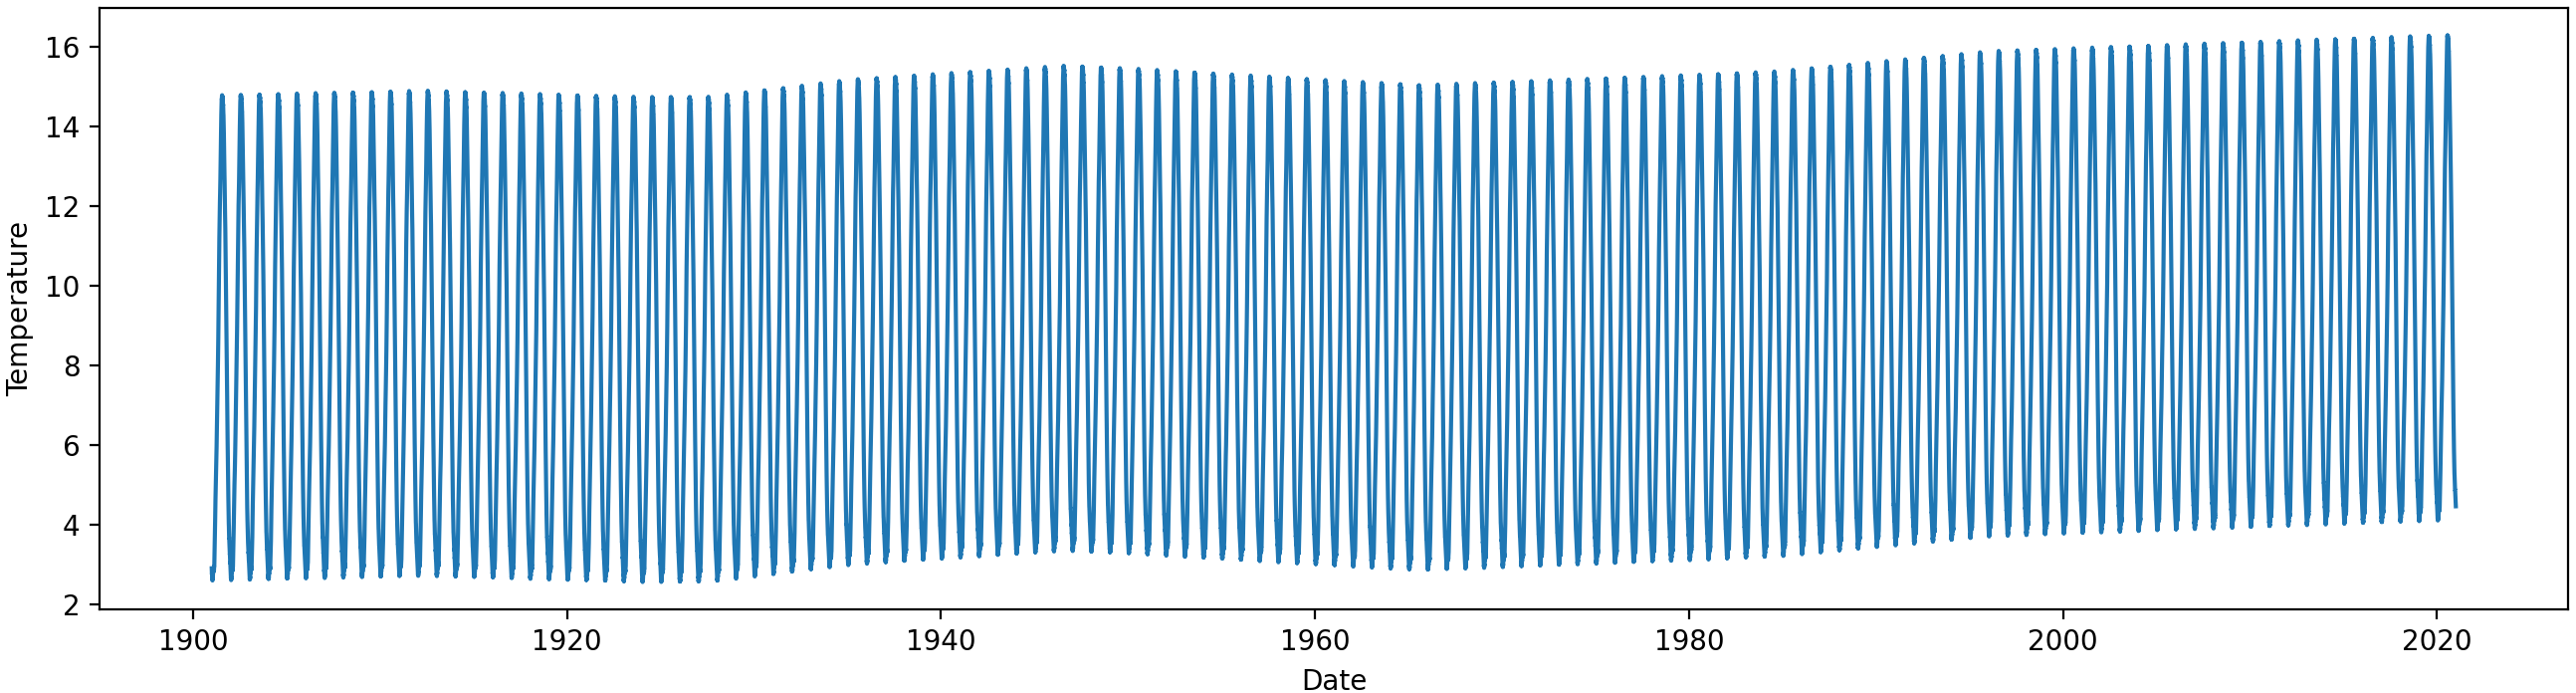
\includegraphics[width=16cm]{wholeyears.png} %[图片大小]{图片路径}
\caption{Temperature of 1901-2020} %图片标题
\end{figure}

\begin{figure}[h]
\centering
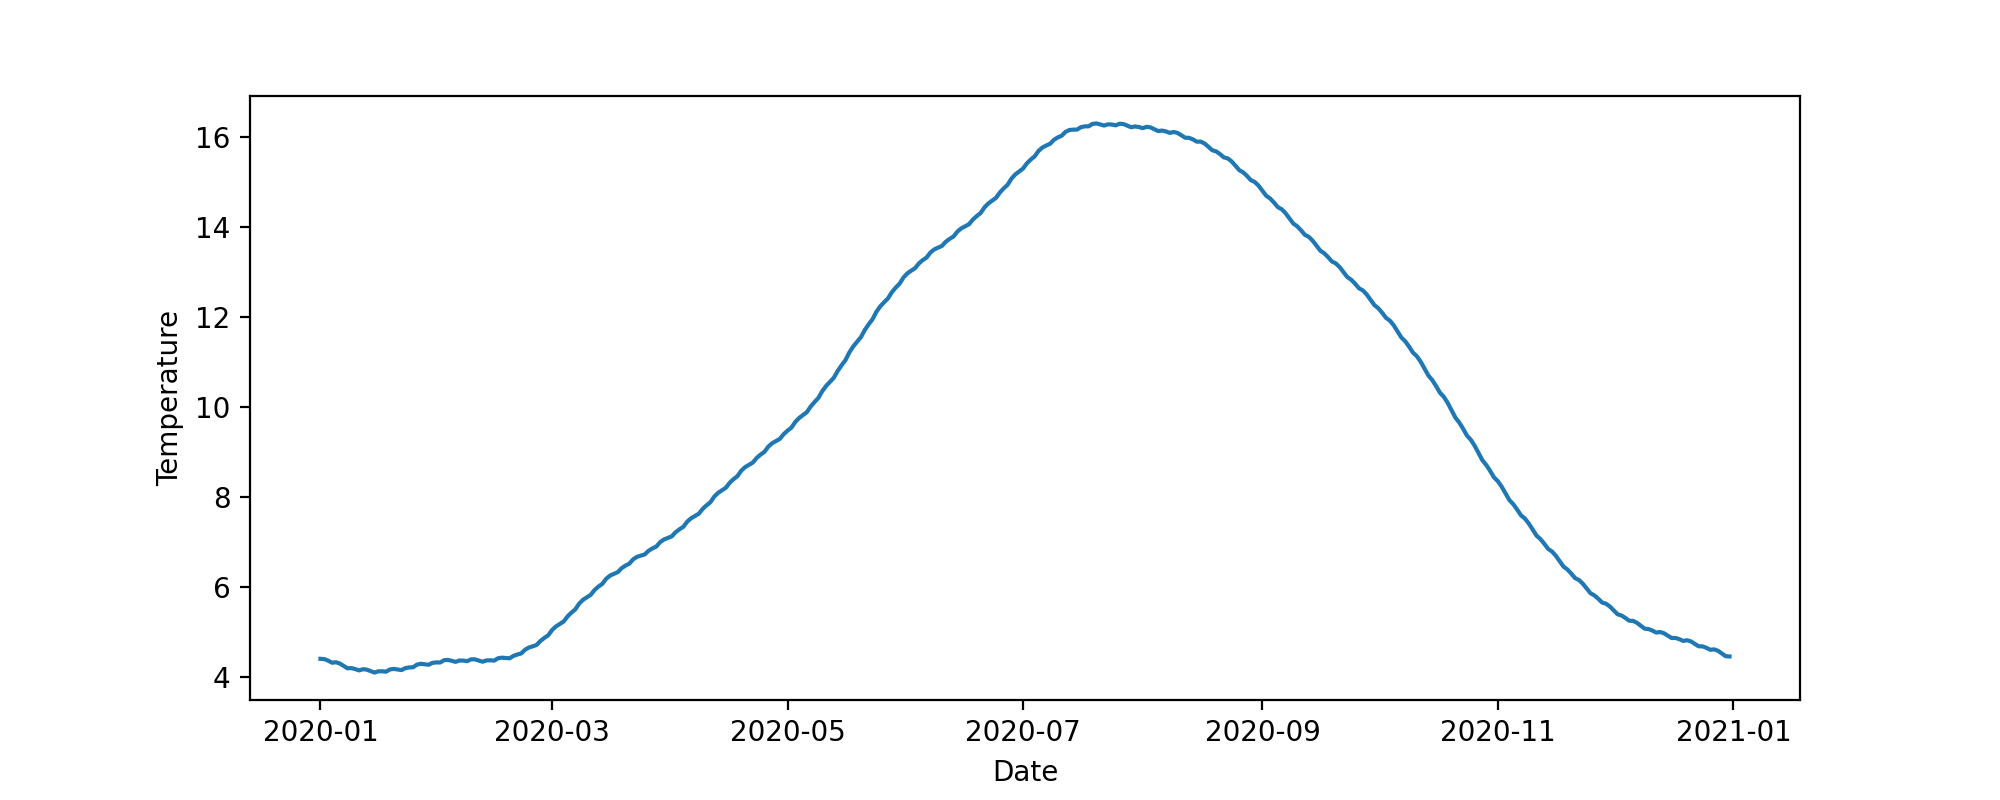
\includegraphics[width=16cm]{year2020.png} %[图片大小]{图片路径}
\caption{Prediction of 2020} %图片标题
\end{figure}

\begin{figure}[h]
\centering
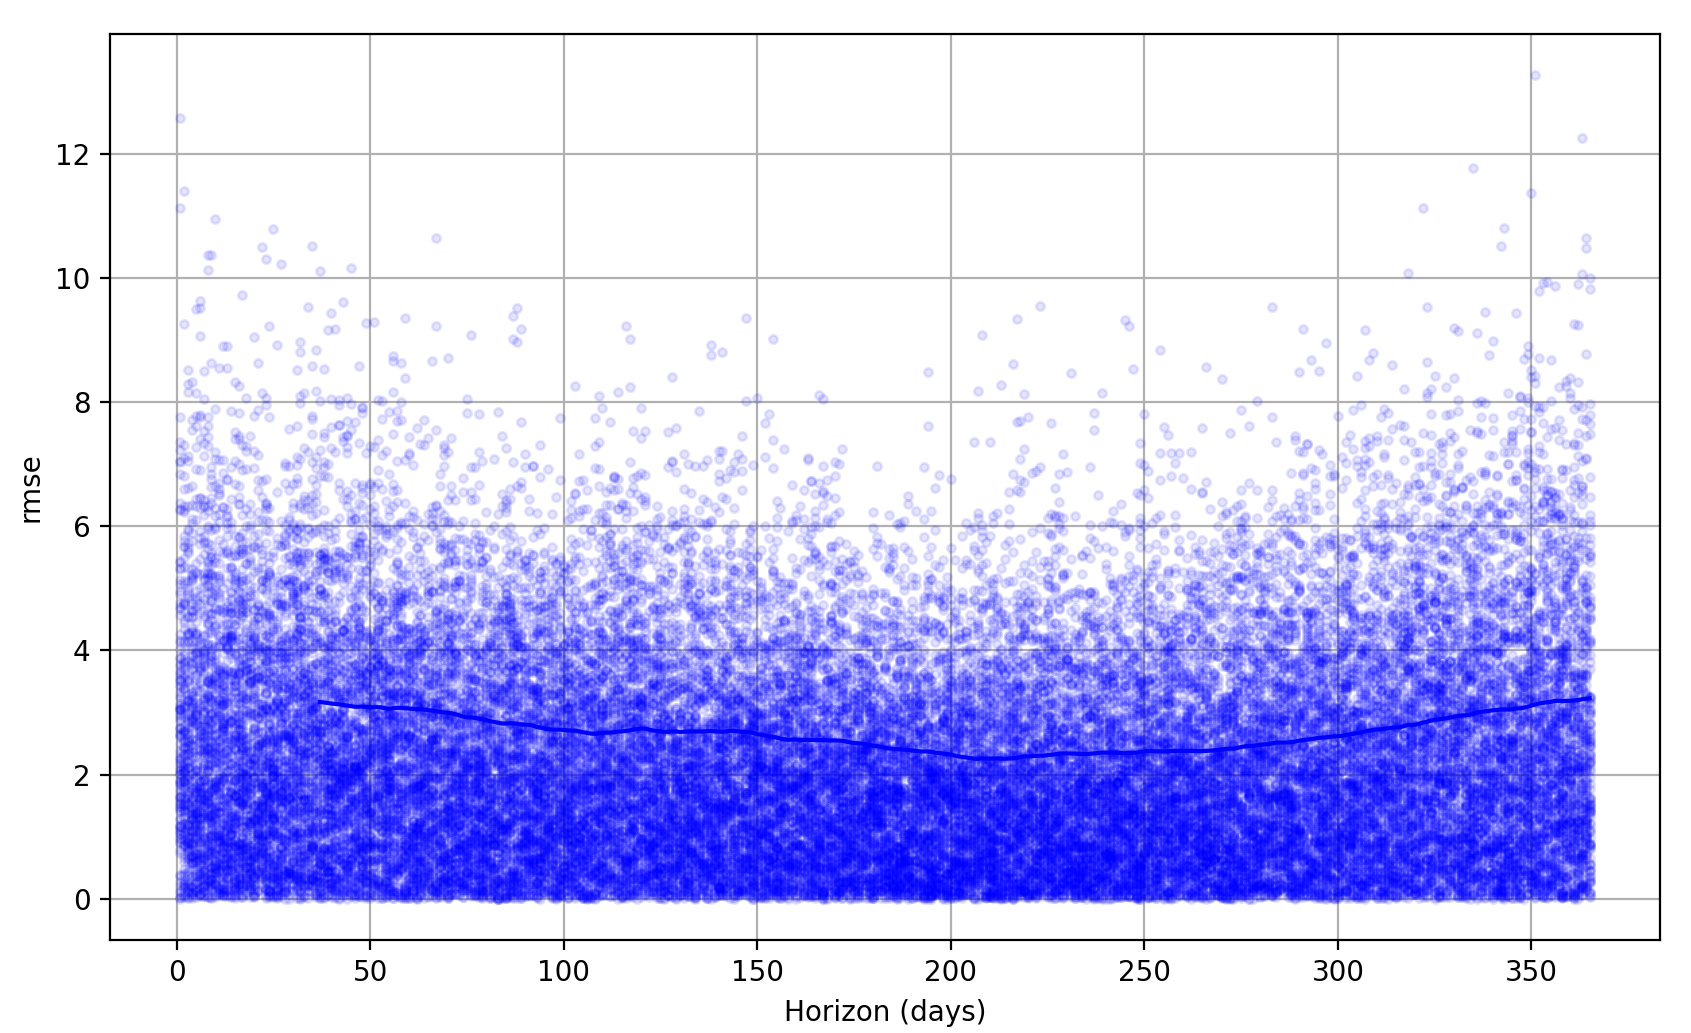
\includegraphics[width=12cm]{rmse.png} %[图片大小]{图片路径}
\caption{RMSE of the prediction} %图片标题
\end{figure}

\begin{figure}[h]
\centering
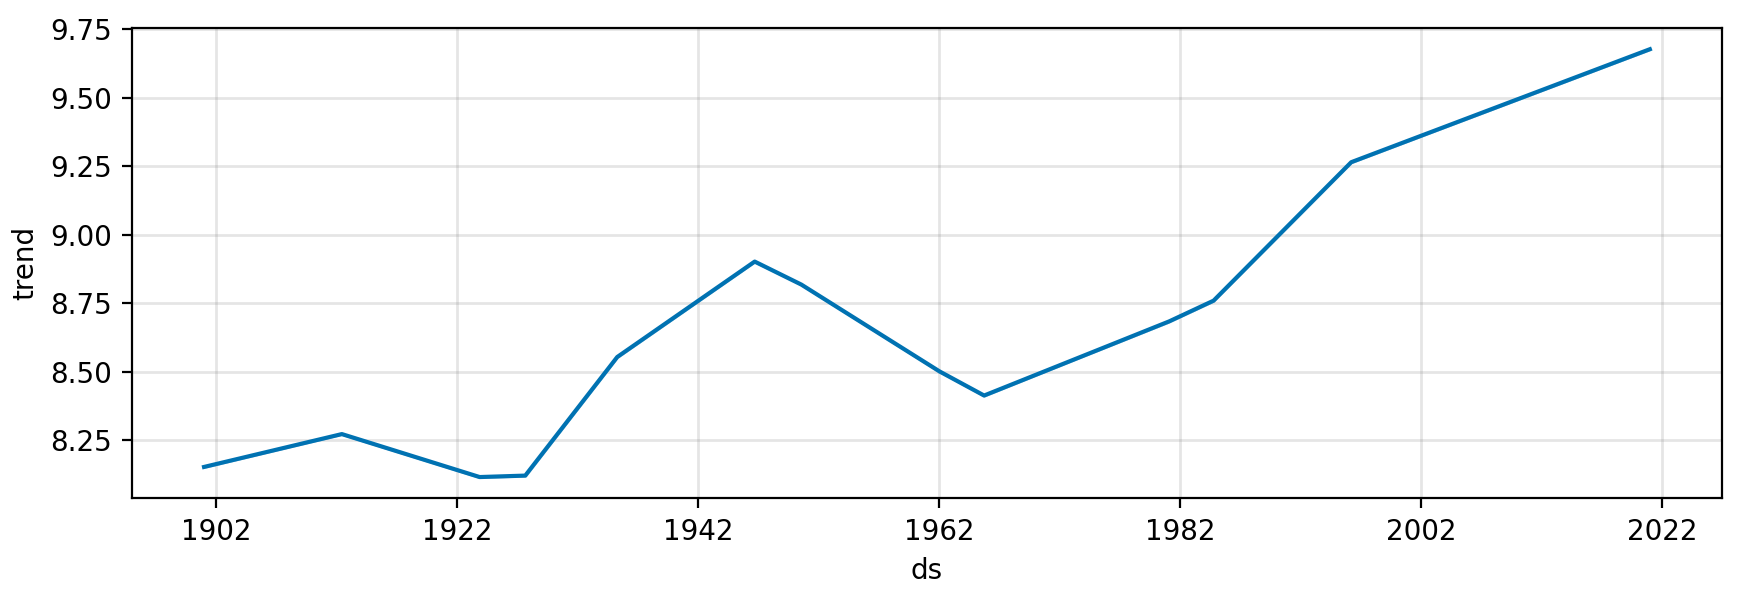
\includegraphics[width=15cm]{trend.png} %[图片大小]{图片路径}
\caption{Trend of average annual temperature} %图片标题
\end{figure}

\end{document}